%%%%%%%%%%%%%%%%%%%%%%%%%%%%%%%%%%%%%%%%%
% Short Sectioned Assignment LaTeX Template Version 1.0 (5/5/12)
% This template has been downloaded from: http://www.LaTeXTemplates.com
% Original author:  Frits Wenneker (http://www.howtotex.com)
% License: CC BY-NC-SA 3.0 (http://creativecommons.org/licenses/by-nc-sa/3.0/)
%%%%%%%%%%%%%%%%%%%%%%%%%%%%%%%%%%%%%%%%%

%----------------------------------------------------------------------------------------
%	PACKAGES AND OTHER DOCUMENT CONFIGURATIONS
%----------------------------------------------------------------------------------------

\documentclass[paper=a4, fontsize=11pt]{scrartcl} % A4 paper and 11pt font size

% ---- Entrada y salida de texto -----

\usepackage[T1]{fontenc} % Use 8-bit encoding that has 256 glyphs
\usepackage[utf8]{inputenc}
%\usepackage{fourier} % Use the Adobe Utopia font for the document - comment this line to return to the LaTeX default

% ---- Idioma --------

\usepackage[spanish, es-tabla]{babel} % Selecciona el español para palabras introducidas automáticamente, p.ej. "septiembre" en la fecha y especifica que se use la palabra Tabla en vez de Cuadro

% ---- Otros paquetes ----

\usepackage{url} % ,href} %para incluir URLs e hipervínculos dentro del texto (aunque hay que instalar href)
\usepackage{amsmath,amsfonts,amsthm} % Math packages
%\usepackage{graphics,graphicx, floatrow} %para incluir imágenes y notas en las imágenes
\usepackage{graphics,graphicx, float} %para incluir imágenes y colocarlas
\usepackage{epstopdf}

% Para hacer tablas comlejas
%\usepackage{multirow}
%\usepackage{threeparttable}

%\usepackage{sectsty} % Allows customizing section commands
%\allsectionsfont{\centering \normalfont\scshape} % Make all sections centered, the default font and small caps

\usepackage{fancyhdr} % Custom headers and footers
\pagestyle{fancyplain} % Makes all pages in the document conform to the custom headers and footers
\fancyhead{} % No page header - if you want one, create it in the same way as the footers below
\fancyfoot[L]{} % Empty left footer
\fancyfoot[C]{} % Empty center footer
\fancyfoot[R]{\thepage} % Page numbering for right footer
\renewcommand{\headrulewidth}{0pt} % Remove header underlines
\renewcommand{\footrulewidth}{0pt} % Remove footer underlines
\setlength{\headheight}{13.6pt} % Customize the height of the header

\numberwithin{equation}{section} % Number equations within sections (i.e. 1.1, 1.2, 2.1, 2.2 instead of 1, 2, 3, 4)
\numberwithin{figure}{section} % Number figures within sections (i.e. 1.1, 1.2, 2.1, 2.2 instead of 1, 2, 3, 4)
\numberwithin{table}{section} % Number tables within sections (i.e. 1.1, 1.2, 2.1, 2.2 instead of 1, 2, 3, 4)

\setlength\parindent{0pt} % Removes all indentation from paragraphs - comment this line for an assignment with lots of text

\newcommand{\horrule}[1]{\rule{\linewidth}{#1}} % Create horizontal rule command with 1 argument of height


%----------------------------------------------------------------------------------------
%	TÍTULO Y DATOS DEL ALUMNO
%----------------------------------------------------------------------------------------

\title{	
\normalfont \normalsize 
\textsc{\textbf{Curso 2016-2017} \\ Grado en Ingeniería Informática \\ Universidad de Granada} \\ [25pt] % Your university, school and/or department name(s)
\horrule{0.5pt} \\[0.4cm] % Thin top horizontal rule
\huge SPSI \\ Práctica 2 \\ % The assignment title
\horrule{2pt} \\[0.5cm] % Thick bottom horizontal rule
}

\author{Carlos Manuel Sequí Sánchez} % Nombre y apellidos

\date{\normalsize\today} % Incluye la fecha actual

%----------------------------------------------------------------------------------------
% DOCUMENTO
%----------------------------------------------------------------------------------------

\begin{document}

\maketitle % Muestra el Título

\newpage %inserta un salto de página

\tableofcontents % para generar el índice de contenidos

\listoffigures

\listoftables

\newpage




%-------------------------------------------------------------------------------------

%-------------------------------------------------------------------------------------

%-------------------------------------------------------------------------------------

%-------------------------------------------------------------------------------------

%-------------------------------------------------------------------------------------

%-------------------------------------------------------------------------------------

%-------------------------------------------------------------------------------------

\section{EJERCICIO 1. Generad, cada uno de vosotros, una clave RSA (que contiene el par de claves) de 768 bits. Para referirnos a ella supondré que se llama nombreRSAkey.pem. Esta clave no es necesario que esté protegida por contraseña.}

Generamos la clave RSA de 768 bits sin protección por contraseña: \\
\textbf{openssl genrsa -out CarlosRSAkey.pem 768}

%-------------------------------------------------------------------------------------

%-------------------------------------------------------------------------------------

%-------------------------------------------------------------------------------------

%-------------------------------------------------------------------------------------

%-------------------------------------------------------------------------------------

%-------------------------------------------------------------------------------------

%-------------------------------------------------------------------------------------

\section{EJERCICIO 2.''Extraed'' la clave privada contenida en el archivo nombreRSAkey.pem a otro archivo que tenga por nombre nombreRSApriv.pem. Este archivo deberá estar protegido por contraseña cifrándolo con AES-128. Mostrad sus valores.}

Extraemos la clave privada en CarlosRSApriv.pem y la protegemos mediante AES-128 introduciéndole la contraseña 0123456789: \\
\textbf{openssl rsa -in CarlosRSAkey.pem -out CarlosRSApriv.pem -outform PEM -aes128}

\begin{figure}[H] %con el [H] le obligamos a situar aquí la figura
	\centering
	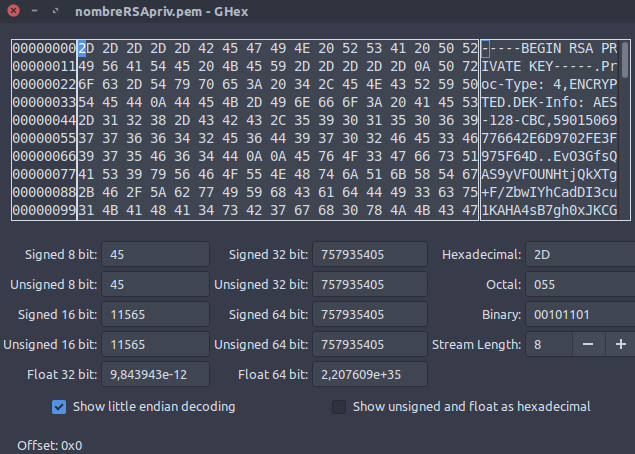
\includegraphics[scale=0.55]{imagenes/CarlosRSApriv} 
	\caption{CarlosRSApriv} \label{etiq}
\end{figure}


\newpage



%-------------------------------------------------------------------------------------

%-------------------------------------------------------------------------------------

%-------------------------------------------------------------------------------------

%-------------------------------------------------------------------------------------

%-------------------------------------------------------------------------------------

%-------------------------------------------------------------------------------------

%-------------------------------------------------------------------------------------

\section{EJERCICIO 3.Extraed en nombreRSApub.pem la clave pública contenida en el archivo nombreRSAkey.pem. Evidentemente nombreRSApub.pem no debe estar cifrado ni protegido. Mostrad sus valores}

Extraemos la clave publica de CarlosRSAkey.pem:
\textbf{openssl rsa -in /home/carlos/\\Escritorio/ETSIIT/SPSI/Prácticas/P2/CarlosRSAkey.pem -outform PEM -pubout -out /home/carlos/\\Escritorio/ETSIIT/SPSI/Prácticas/P2/CarlosRSApub.pem}

\begin{figure}[H] %con el [H] le obligamos a situar aquí la figura
	\centering
	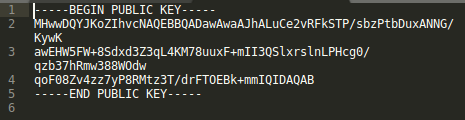
\includegraphics[scale=0.55]{imagenes/CarlosRSApub} 
	\caption{CarlosRSApub} \label{etiq}
\end{figure}


\newpage



%-------------------------------------------------------------------------------------

%-------------------------------------------------------------------------------------

%-------------------------------------------------------------------------------------

%-------------------------------------------------------------------------------------

%-------------------------------------------------------------------------------------

%-------------------------------------------------------------------------------------

%-------------------------------------------------------------------------------------

\section{EJERCICIO 4.Intentad cifrar input.bin con vuestras claves públicas. Explicad el resultado. }

Ciframos input.bin con clave pública \\
\textbf{openssl rsautl -encrypt -pubin -inkey /home/carlos/Escritorio/ETSIIT/SPSI/\\Prácticas/P2/CarlosRSApub.pem -in /home/carlos/Escritorio/ETSIIT/SPSI/\\Prácticas/P2/input.bin -out /home/carlos/Escritorio/ETSIIT/SPSI/\\Prácticas/P2/inputEncriptado.bin} \\

No está permitido cifrar input.bin ya que este tiene un tamaño de 1024 bits y la clave es de 768 bits, por tanto llegamos a la conclusión
de que no es posible cifrar un fichero que tiene mayor tamaño que la clave que se quiere utilizar para cifrar.
Esto es porque RSA es cifrado de flujo y no por bloques, por lo que necesita que la clave sea igual de grande que el mensaje.



%-------------------------------------------------------------------------------------

%-------------------------------------------------------------------------------------

%-------------------------------------------------------------------------------------

%-------------------------------------------------------------------------------------

%-------------------------------------------------------------------------------------

%-------------------------------------------------------------------------------------

%-------------------------------------------------------------------------------------

\section{EJERCICIO 5.Diseñad un cifrado híbrido, con RSA como criptosistema asimétrico. }

\begin{enumerate}
	\item Elijo el sistema simétrico DES CBC.
	\item Generamos sessionkey.txt
		\begin{itemize}
			\item Para generar la cadena aleatoria utilizamos openssl rand, con un tamaño 8, ya que el tamaño de clave para DES es de 16 bytes:\\
			\textbf{openssl rand -hex 8 > /home/carlos/Escritorio/ETSIIT/\\SPSI/Prácticas/P2/sessionkey.txt}
			\item Establecemos el sistema simétrico utilizado en la segunda línea del fichero \\
			\textbf{echo "-des-cbc" >> /home/carlos/Escritorio/ETSIIT/SPSI/\\Prácticas/P2/sessionkey.txt}
		\end{itemize}
	
		\begin{figure}[H] %con el [H] le obligamos a situar aquí la figura
			\centering
			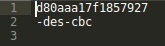
\includegraphics[scale=1]{imagenes/sessionkey} 
			\caption{archivo sessionkey} \label{etiq}
		\end{figure}
	\item Ciframos sessionkey con la clave pública del receptor: \\
		\textbf{openssl rsautl -encrypt -pubin -inkey\\ /home/carlos/Escritorio/ETSIIT/SPSI/\\Prácticas/P2/CarlosRSApub.pem -in /home/carlos/Escritorio/ETSIIT/SPSI/\\Prácticas/P2/sessionkey.txt -out sessionkeyEncrypted.txt}
		
		\begin{figure}[H] %con el [H] le obligamos a situar aquí la figura
			\centering
			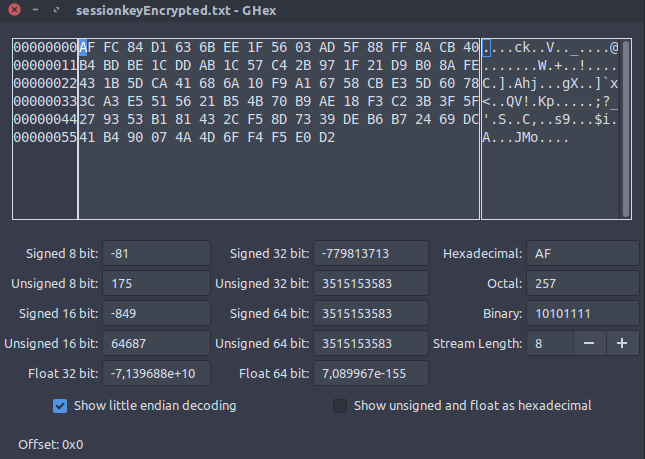
\includegraphics[scale=0.55]{imagenes/sessionkeyEncrypted} 
			\caption{sessionkey encriptado} \label{etiq}
		\end{figure}
		
	\item Ciframos el mensaje con DES CBC con clave semidébil:\\
		\textbf{openssl enc -des-cbc -pass\\ file:/home/carlos/Escritorio/ETSIIT/SPSI/\\Prácticas/P2/sessionkey.txt -iv 1231231231231231 -in /home/carlos/Escritorio/\\ETSIIT/SPSI/Prácticas/P2/input.bin -out /home/carlos/Escritorio/ETSIIT/\\SPSI/Prácticas/P2/inputEncriptado.bin}
		
		\begin{figure}[H] %con el [H] le obligamos a situar aquí la figura
			\centering
			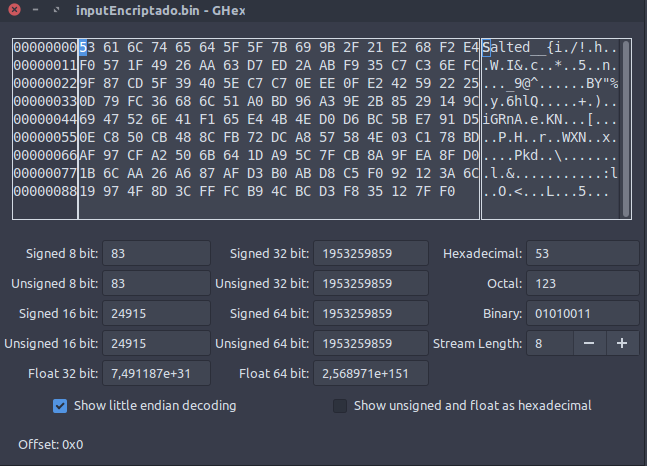
\includegraphics[scale=0.55]{imagenes/inputEncriptado} 
			\caption{input.bin encriptado} \label{etiq}
		\end{figure}
\end{enumerate}

\newpage

%-------------------------------------------------------------------------------------

%-------------------------------------------------------------------------------------

%-------------------------------------------------------------------------------------

%-------------------------------------------------------------------------------------

%-------------------------------------------------------------------------------------

%-------------------------------------------------------------------------------------

%-------------------------------------------------------------------------------------

\section{EJERCICIO 6.Utilizando el criptosistema híbrido diseñado, cada uno debe cifrar el archivo input.bin con su clave pública para, a continuación, descifrarlo con la clave privada. comparad el resultado con el archivo original.}

Mensaje original que se desea enviar desde el emisor hasta el receptor.\\

\begin{figure}[H] %con el [H] le obligamos a situar aquí la figura
	\centering
	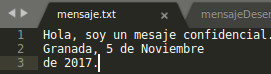
\includegraphics[scale=1]{imagenes/mensajeOriginalE7} 
	\caption{mensaje original} \label{etiq}
\end{figure}

\begin{enumerate}
	\item Creamos el archivo sessionkey.\\
		\begin{itemize}
			\item -Para generar la cadena aleatoria utilizamos openssl rand, con un tamaño 8, ya que el tamaño de clave para DES es de 16 bytes:\\
			\textbf{openssl rand -hex 8 > /home/carlos/Escritorio/ETSIIT/SPSI/\\Prácticas/P2/ej7/sessionkey.txt}
			
			\item -Establecemos el sistema simétrico utilizado en la segunda línea del fichero\\
			\textbf{echo "-des-cbc" >> /home/carlos/Escritorio/ETSIIT/SPSI/\\Prácticas/P2/ej7/sessionkey.txt}
		\end{itemize}
	
	\begin{figure}[H] %con el [H] le obligamos a situar aquí la figura
		\centering
		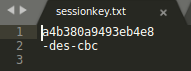
\includegraphics[scale=1]{imagenes/sessionkeyE7} 
		\caption{archivo sessionkey} \label{etiq}
	\end{figure}
	
	\item Ciframos el mensaje con el criptosistema diseñado (DES-CBC) y utilizando como clave el archivo sessionkey generado: \\
		\textbf{openssl enc -des-cbc -pass file:/home/carlos/Escritorio/ETSIIT/SPSI/\\Prácticas/P2/ej7/sessionkey.txt -iv 1231231231231231 -in /home/carlos/Escritorio/\\ETSIIT/SPSI/Prácticas/P2/ej7/mensaje.txt -out /home/carlos/Escritorio/\\ETSIIT/SPSI/Prácticas/P2/ej7/mensajeEncriptado.txt}
		
		\begin{figure}[H] %con el [H] le obligamos a situar aquí la figura
			\centering
			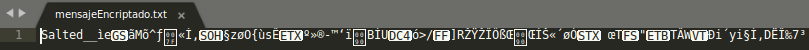
\includegraphics[scale=0.60]{imagenes/mensajeEncriptadoE7} 
			\caption{mensaje cifrado} \label{etiq}
		\end{figure}
	
	\item Ciframos el sessionkey con la clave publica del receptor. \\
	\textbf{openssl rsautl -encrypt -pubin -inkey\\ /home/carlos/Escritorio/ETSIIT/SPSI/Prácticas/P2/\\ej7/CarlosRSApub.pem -in /home/carlos/Escritorio/ETSIIT/SPSI/Prácticas/P2/\\ej7/sessionkey.txt -out /home/carlos/Escritorio/ETSIIT/SPSI/Prácticas/P2/\\ej7/sessionkeyEncrypted.txt}
	
	\begin{figure}[H] %con el [H] le obligamos a situar aquí la figura
		\centering
		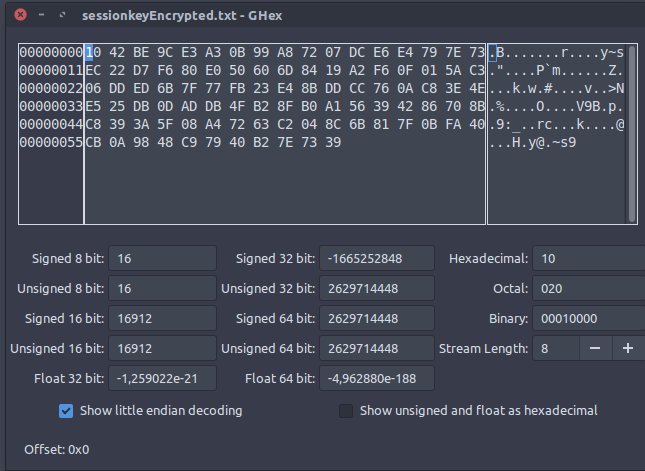
\includegraphics[scale=0.55]{imagenes/sessionkeyEncryptedE7} 
		\caption{sessionkey encriptado} \label{etiq}
	\end{figure}
	
	\item Enviamos al receptor esos dos archivos encriptados, tanto la sessionkey como el propio mensaje.
	
	\item El receptor con su clave privada desencripta el sessionkey introduciendo la contraseña adecuada \\
	\textbf{	openssl rsautl -decrypt -inkey \\ /home/carlos/Escritorio/ETSIIT/SPSI/Prácticas/P2/\\ej7/CarlosRSApriv.pem -in /home/carlos/Escritorio/ETSIIT/SPSI/Prácticas/P2/\\ej7/sessionkeyEncrypted.txt -out /home/carlos/Escritorio/ETSIIT/SPSI/Prácticas/\\P2/ej7/sessionkeyDesencriptado.txt}
	
	\begin{figure}[H] %con el [H] le obligamos a situar aquí la figura
		\centering
		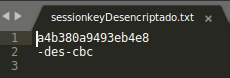
\includegraphics[scale=1]{imagenes/sessionkeyDesencriptadoE7} 
		\caption{sessionkey desencriptado} \label{etiq}
	\end{figure}
	
		\item Una vez ha desencriptado el sessionkey se genera un archivo sessionkeyDesencriptado que usaremos para
		desencriptar el mensaje original.\\
		\textbf{openssl des-cbc -d -pass file:/home/carlos/Escritorio/ETSIIT/SPSI/\\Prácticas/P2/ej7/sessionkeyDesencriptado.txt -iv 1231231231231231 -in\\ /home/carlos/Escritorio/ETSIIT/SPSI/\\Prácticas/P2/ej7/mensajeEncriptado.txt -out /home/carlos/Escritorio/ETSIIT/SPSI/\\Prácticas/P2/ej7/mensajeDesencriptado.txt}
		
		\begin{figure}[H] %con el [H] le obligamos a situar aquí la figura
			\centering
			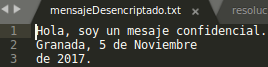
\includegraphics[scale=1]{imagenes/mensajeDesencriptadoE7} 
			\caption{mensaje desencriptado por el receptor} \label{etiq}
		\end{figure}
\end{enumerate}


\newpage


%-------------------------------------------------------------------------------------

%-------------------------------------------------------------------------------------

%-------------------------------------------------------------------------------------

%-------------------------------------------------------------------------------------

%-------------------------------------------------------------------------------------

%-------------------------------------------------------------------------------------

%-------------------------------------------------------------------------------------


\section{EJERCICIO 7.Generad un archivo stdECparam.pem que contenga los parámetros públicos de una de las curvas elípticas contenidas en las transparencias de teoría. Si no lográis localizarlas haced el resto de la práctica con una curva cualquiera a vuestra elección de las disponibles en OpenSSL. Mostrad los valores.}


Generamos los parámetros de la curva:\\
\textbf{openssl ecparam -name brainpoolP192r1 -out\\ /home/carlos/Escritorio/ETSIIT/SPSI/Prácticas/P2/ej8/stdECparam.pem}

\begin{figure}[H] %con el [H] le obligamos a situar aquí la figura
	\centering
	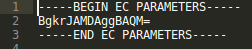
\includegraphics[scale=1]{imagenes/stdECparam} 
	\caption{Parámetros curva elíptica} \label{etiq}
\end{figure}


%-------------------------------------------------------------------------------------

%-------------------------------------------------------------------------------------

%-------------------------------------------------------------------------------------

%-------------------------------------------------------------------------------------

%-------------------------------------------------------------------------------------

%-------------------------------------------------------------------------------------

%-------------------------------------------------------------------------------------


\section{EJERCICIO 8. Generad cada uno de vosotros una clave para los parámetros anteriores. La clave se almacenará en nombreECkey.pem y no es necesario protegerla por contraseña. }

Generamos la clave para esos parámetros:\\
\textbf{openssl ecparam -in /home/carlos/Escritorio/\\ETSIIT/SPSI/Prácticas/P2/ej8/stdECparam.pem -genkey -noout \\-out /home/carlos/Escritorio/ETSIIT/SPSI/Prácticas/P2/\\ej8/CarlosECkey.pem}

\begin{figure}[H] %con el [H] le obligamos a situar aquí la figura
	\centering
	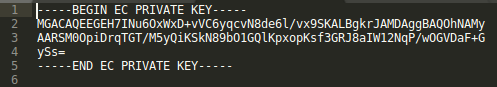
\includegraphics[scale=0.8]{imagenes/CarlosECkey} 
	\caption{Clave generada para los parámetros} \label{etiq}
\end{figure}

%-------------------------------------------------------------------------------------

%-------------------------------------------------------------------------------------

%-------------------------------------------------------------------------------------

%-------------------------------------------------------------------------------------

%-------------------------------------------------------------------------------------

%-------------------------------------------------------------------------------------

%-------------------------------------------------------------------------------------


\section{EJERCICIO 9.''Extraed'' la clave privada contenida en el archivo nombreECkey.pem a otro archivo que tenga por nombre nombreECpriv.pem. Este archivo deberá estar protegido por contraseña cifrándolo con 3DES. Mostrad sus valores.}
Sacamos la privada y la protegemos con la clave 0123456789: \\
\textbf{openssl ec -in /home/carlos/Escritorio/ETSIIT/\\SPSI/Prácticas/P2/ej8/CarlosECkey.pem -out /home/carlos/Escritorio/\\ETSIIT/SPSI/Prácticas/P2/ej8/CarlosECpriv.pem -outform PEM -des3}

\begin{figure}[H] %con el [H] le obligamos a situar aquí la figura
	\centering
	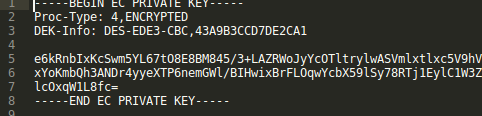
\includegraphics[scale=0.8]{imagenes/CarlosECpriv} 
	\caption{Clave privada cifrada con 3DES} \label{etiq}
\end{figure}

%-------------------------------------------------------------------------------------

%-------------------------------------------------------------------------------------

%-------------------------------------------------------------------------------------

%-------------------------------------------------------------------------------------

%-------------------------------------------------------------------------------------

%-------------------------------------------------------------------------------------

%-------------------------------------------------------------------------------------


\section{EJERCICIO 10.Extraed en nombreECpub.pem la clave pública contenida en el archivo nombreECkey.pem. Como antes	nombreECpub.pem no debe estar cifrado ni protegido. Mostrad sus valores.}
Sacamos la pública:\\
\textbf{openssl ec -in /home/carlos/Escritorio/ETSIIT/\\SPSI/Prácticas/P2/ej8/CarlosECkey.pem -pubout -out /home/\\carlos/Escritorio/ETSIIT/SPSI/Prácticas/P2/ej8/CarlosECpub.pem}

\begin{figure}[H] %con el [H] le obligamos a situar aquí la figura
	\centering
	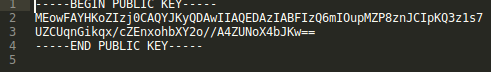
\includegraphics[scale=0.8]{imagenes/CarlosECpub} 
	\caption{Clave pública} \label{etiq}
\end{figure}


\newpage
%------------------------------------------------




\end{document}
